\documentclass[12pt,ngerman]{article}
\usepackage{tabularx,amsmath,boxedminipage,graphicx}
\usepackage{babel}
%\usepackage[ansinew]{inputenc}
\usepackage[utf8]{inputenc}
%\usepackage{url}
\usepackage[T1]{fontenc}
%\usepackage[autostyle=true]{csquotes}
%\usepackage{commath}
%\usepackage[varg]{txfonts}
%\usepackage{hyperref}
%\usepackage{siunitx}
%\usepackage{bbm}
%\usepackage{listings}
%\usepackage{cite}
%\usepackage{graphicx}
%\usepackage{esdiff}
%\usepackage{esvect}
%\usepackage[toc,page]{appendix}
\graphicspath{{figs/}}
\bibliographystyle{unsrt}



\begin{document}
	\tableofcontents
	\newpage
	\section{Messung analoger Größen}
	\subsection{a}
Zunächst muss der Strom der Driftkammer in abhägigkeit von der Hochspannung eingetragen werden. Mittels ohmsches Gesetzt ist die Spannung in Strom auszurechnen. 
\begin{align*}
U&=R.I \Leftrightarrow\\
I&=\frac{U}{R}\\
\Delta I&=\frac{\Delta U}{R}
\end{align*}
Hierbei ist $R=1M\Omega$ angenommen.
Die gemessene Werte lauten:
\begin{table}[h]
	\centering
	\begin{tabular}{c c c c}
	$U_{\text{Drift}}$/kV& $\Delta U_{\text{Drift}}$/V&$I$/nA&$\Delta I$/nA\\\hline
	2.105&	0.0421&	5&	0.25\\
	2.204&	0.0440&	6&	0.25\\
	2.304&	0.0460&	7&	0.25\\
	2.402&	0.0480&	8&	0.5\\
	2.502&	0.0500&	9&	1\\
	2.602&	0.0520&	10&	1\\
	2.707&	0.0541&	12&	1.5\\
	2.805&	0.0561&	17&	3\\
	2.907&	0.0581&	25&	5\\
	2.95&	0.059&	32&	6\\
	2.997&	0.0599&	45&	10\\
	\end{tabular}
	 \caption{Messunge der Spannung ohne Quelle. Zu beachten ist, dass die $\Delta U_{\text{Drift}}$ als 20\% von $U_{\text{Drift}}$ angenommen worden ist. Die dazugehöroge Diagramm ist in Abbildung \ref{figohne} zu finden.}
\end{table}
\begin{figure}[htbp]
\centering
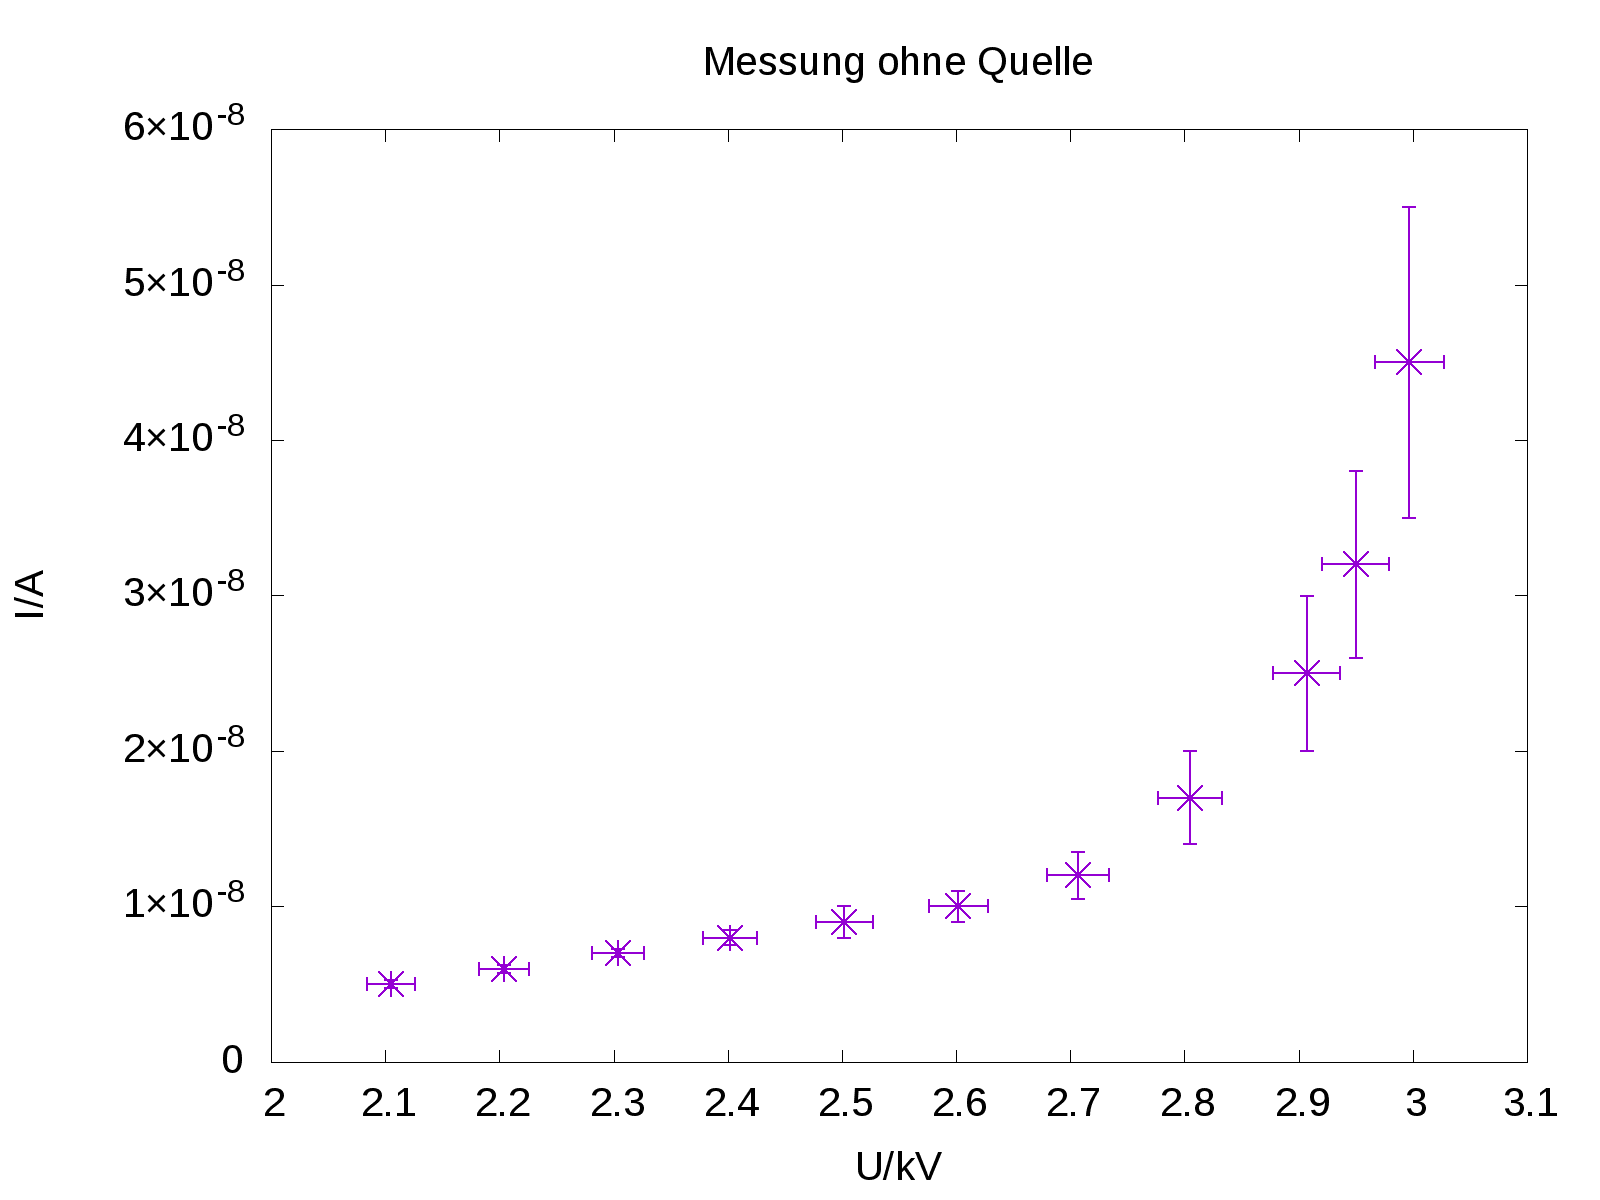
\includegraphics[width=0.45\textheight]{ohne.png}
\caption{ Es ist auf diese Diagramm zu sehen, dass je höher Strom geht, desto höhere schwankungen zu folge ist.}
\label{figohne}
\end{figure}
\begin{table}[h]
	\centering
	\begin{tabular}{c c c c}
		$U_{\text{Drift}}$/kV& $\Delta U_{\text{Drift}}$/V&$I$/nA&$\Delta I$/nA\\\hline
	2.099&	0.0419&	9&	0.5\\
	2.202&	0.0440&	10&	0.5\\
	2.306&	0.0461&	15&	0.5\\
	2.405&	0.0481&	24&	1\\
	2.507&	0.0501&	40&	2\\
	2.601&	0.0520&	71&	35\\
	2.704&	0.0540&	230&	5\\
	2.803&  0.0560&	250&	10\\
	2.906&	0.0581&	535&	20\\
	2.953&	0.0590&	750&	35\\
	2.989&	0.0597&	1450&	35\\
	\end{tabular}
	\caption{Messunge der Spannung mit Quelle. Zu beachten ist, dass die $\Delta U_{\text{Drift}}$ als 20\% von $U_{\text{Drift}}$ angenommen worden ist. Die dazugehöroge Diagramm ist in Abbildung \ref{figmit} zu finden.}
\end{table}
\begin{figure}[htbp]
	\centering
	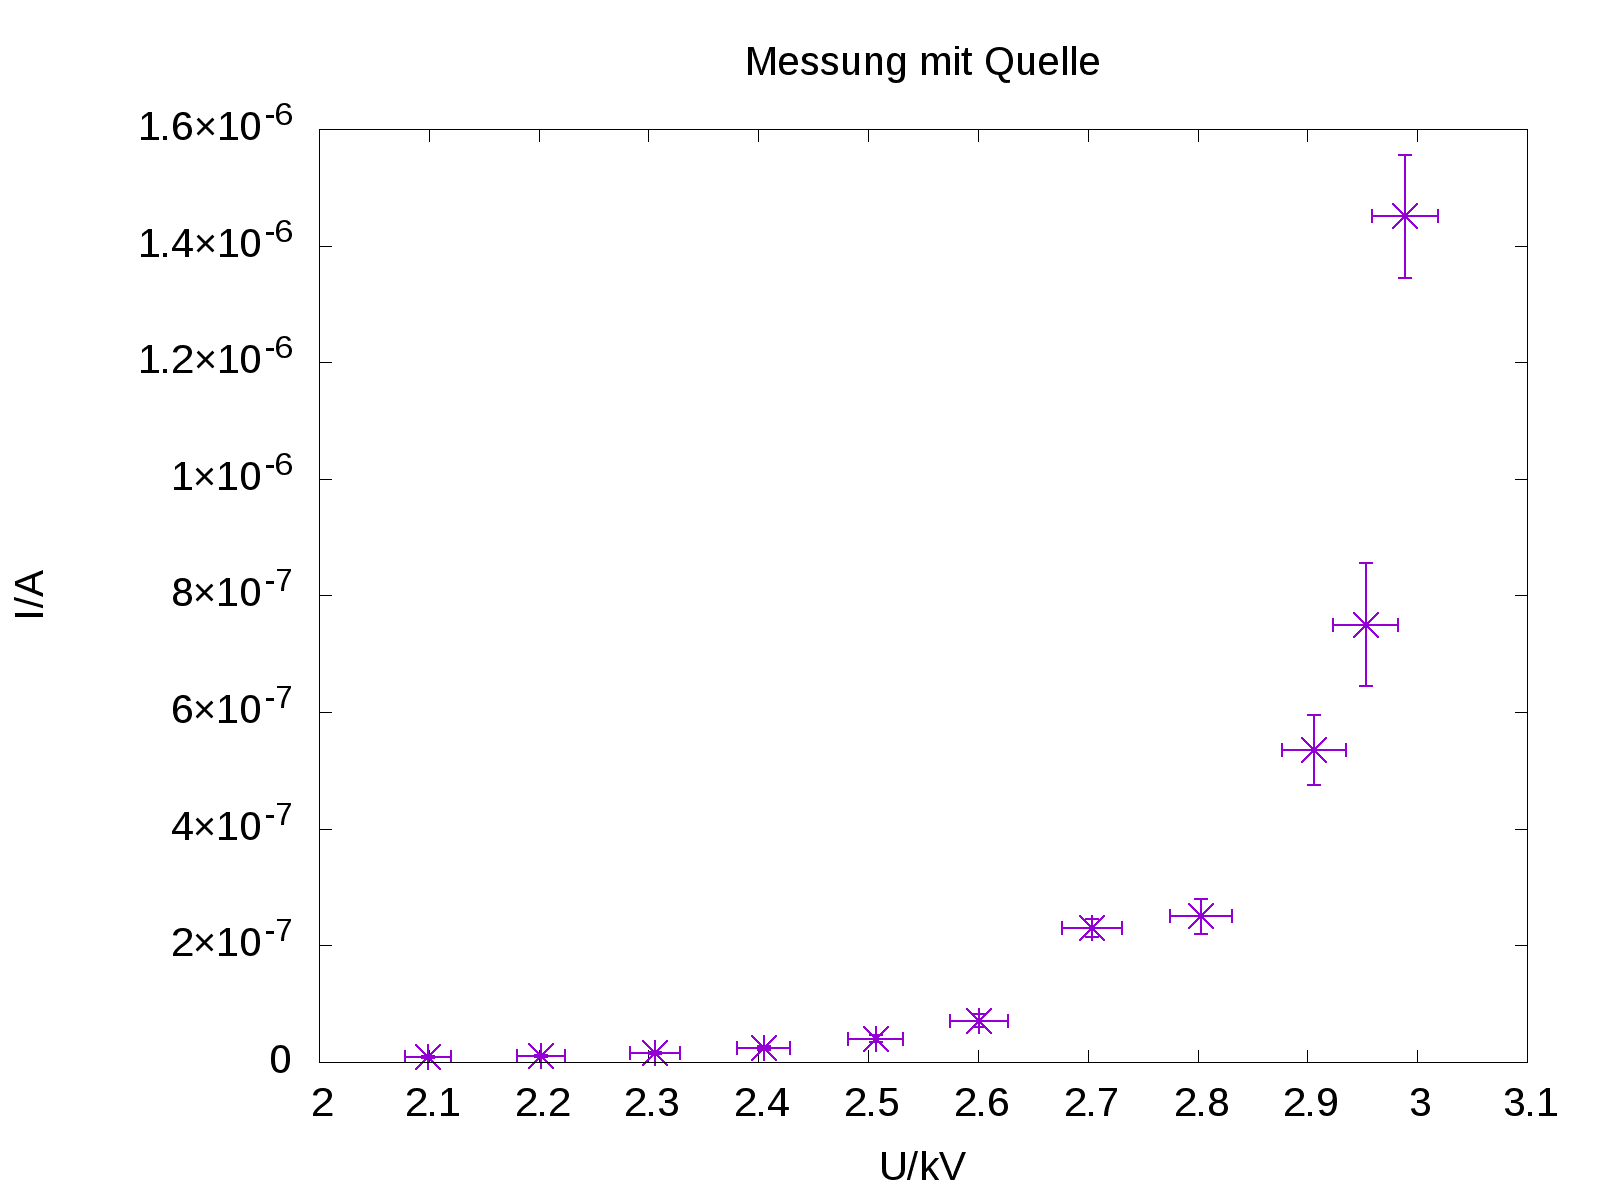
\includegraphics[width=0.45\textheight]{mit.png}
	\caption{ Es ist auf diese Diagramm zu sehen, dass je höher Strom geht, desto höhere schwankungen zu folge ist.}
	\label{figmit}
\end{figure}
\subsection{b}
Nun ist die analoge ausganssignale von Driftkammer und Szintillator auf dem Oszilloskop zu sehen.
 
\end{document}